\documentclass[10pt]{ctexart}
\usepackage{morelull}
\usepackage{enumerate}
\usepackage{bm}
\usepackage{makecell}
\usepackage{xcolor}
\usepackage{graphicx}
\usepackage{subfigure}
\usepackage{framed}%包中有添加文字背景色命令shaded
\colorlet{shadecolor}{MaterialBlue50}
\usepackage{tabularx}
\usepackage{multicol}  
\usepackage{multirow}
\usepackage{indentfirst}
\usepackage{amsmath,amssymb,amsthm,bm,bbding,pifont,dsfont}
\usepackage{mathtools}
\newcommand{\abs}[1]{\left| #1 \right|}
\usepackage{caption}
\captionsetup[figure]{labelfont={bf},labelformat={default},labelsep=period,name={图}}
%定义选择题选项
\newcommand{\onech}[4]{
\renewcommand\arraystretch{1.4}
\begin{tabularx}{\linewidth}{XXXX}
\setlength\tabcolsep{0pt}
(A) #1 & (B) #2 & (C) #3 & (D) #4 \\
\end{tabularx}
\unskip \unskip}
\newcommand{\twoch}[4]{
\renewcommand\arraystretch{1.4}
\begin{tabularx}{\linewidth}{XX}
\setlength\tabcolsep{0pt}
(A) #1 & (B) #2 \\
(C) #3 & (D) #4
\end{tabularx}
\unskip \unskip}

\title{模型研究系列 \quad 费马点问题}
\author{一粒沙整理\\安徽省霍邱县龙潭中学}
\date{\today}



\begin{document}
\maketitle
\tableofcontents


\section{什么是费马点问题?}
有甲乙丙三个村庄,要在中间处建一个供水站向三地送水,现要确定供水站的位置以使所需管道总长最小?将此问题用数学模型抽象出来即为:\textcolor{cyan}{在如下图的$\triangle ABC$(3个内角均小于$120^\circ$)中确定一点$P$,使$P$到三个顶点的距离之和$PA+PB+PC$最小}.

	\begin{center}
		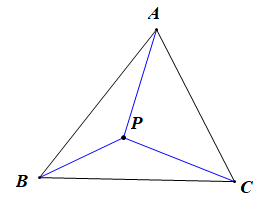
\includegraphics[scale=0.6]{figure/feimadian01}
	\end{center}

该问题中符合条件的点$P$,我们把它叫做\textcolor{red}{费马点}。所谓的“费马点”就是法国著名业余数学家费马在给数学朋友的一封信中提出关于三角形的一个有趣问题:“在三角形所在平面上,求一点,使该点到三角形三个顶点距离之和最小”。让朋友思考,并自称已经证明了,人们称这个点为“费马点”。

\section{费马点问题的求解方法}
【分析】关于求几何最值问题,我们一般可以借助以下两个公理来处理:\textcolor{blue}{两点之间线段最短,点到直线的连线中垂线段最短,作对称化折线段为直线段,确定动点轨迹求最值}等。

因此,在上述问题中要想办法把$PA,PB,PC$这三条分散的线段转化为连续的折线,然后借助两点之间线段最短找到符合条件的点$P$.在解决几何问题过程中,我们常借助于\textcolor{red}{对称变换、平移变换和旋转变换},本题牵涉三条线段,因此我们可以考虑旋转变换。

【 求解方法一】 \textcolor{red}{旋转法}

\begin{center}
	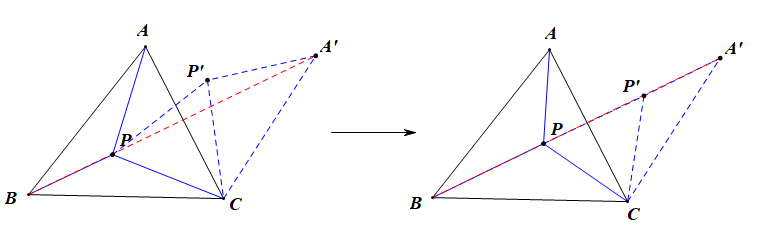
\includegraphics[scale=0.6]{figure/feimadian02}
\end{center}

{\kaishu\color{blue}如图,将$\triangle ACP$绕点$C$\textcolor{red}{顺时针旋转$60^\circ$}得到$\triangle A'CP'$,则$\triangle ACP \cong \triangle A'CP'$,有$CP=CP',AP=A'P',\angle PCP'=\angle ACA'=60^\circ$.所以$\triangle PCP'$是等边三角形.因为$PA+PB+PC=A'P'+PB+PP'\geqslant A'B$,$\therefore$当点$B,P,P',A'$共线时,$PA+PB+PC$最小,如图所示,最小值为$A'B$.

此时,$\angle BPC=180^\circ-\angle CPP'=120^\circ,\angle APC=\angle A'P'C=120^\circ,\angle ABP=360^\circ-\angle BPC-\angle APC=120^\circ$}.

但在这里有一个小小的要求,细心的同学会发现,这个图成立的必要条件是$\angle BAC<120^\circ$,若$\angle BAC \geqslant 120^\circ$,这个图就不是这个图了,会长成这个样子:

\begin{center}
	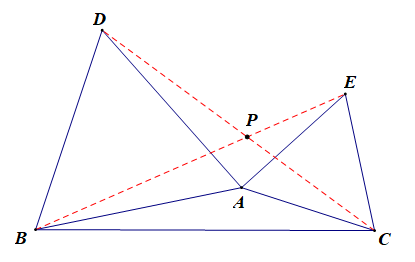
\includegraphics[scale=0.6]{figure/feimadian04}
\end{center}

此时$CD$与$BE$交点$P$点还是我们的费马点吗?显然$P$点到$A,B,C$距离之和大于$A$点到$A,B,C$距离之和,所以咧?是的,你想得没错,此时三角形的费马点就是$A$点!当然这种情况不会考的,就不多说了.



由以上过程我们总结一下费马点的定义及其性质:
\begin{custom}{费马点定义及结论}{}
{\kaishu\color{blue}	数学上称,到三角形三个顶点距离之和最小的点为费马点。
	
	费马点结论:
	
	\ding{192}若三角形有一个内角大于或等于$120^\circ$,这个内角的顶点就是费马点;
	
	\ding{193}若三个内角均小于$120^\circ$,则在三角形内部对三边张角均为$120^\circ$的点是三角形的费马点;
	
	\ding{194}等边三角形的费马点是重心.}
\end{custom}

可以进一步对上述图形进行研究:

\begin{center}
	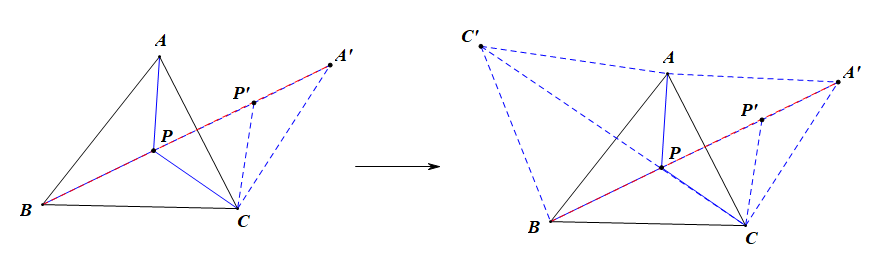
\includegraphics[scale=0.6]{figure/feimadian03}
\end{center}

连接$AA'$,我们发现$\triangle ACA'$为等边三角形,点$P$在$A'B$上,同理,我们可以得到等边$\triangle AC'B$.点$P$也在$CC'$上,因此,我们可以\textcolor{red}{以三角形任意两边为边构造等边三角形,相应连线的交点即为费马点}.下面我们从这个角度再来研究费马点问题。

【 求解方法二】 \textcolor{red}{构造等边三角形法}

\begin{center}
	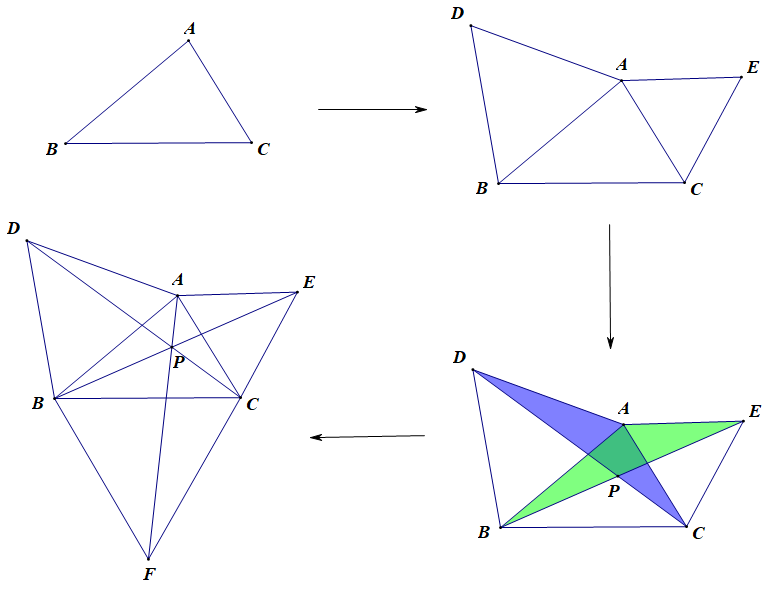
\includegraphics[scale=0.6]{figure/feimadian05}
\end{center}

{\kaishu\color{blue}如图,分别以$\triangle ABC$中的边$AB,AC$为边,作等边$\triangle ABD$,等边$\triangle ACE$,连接$CD,BE$,即有一组手拉手全等({\kaishu\color{red}什么是手拉手?有哪些重要的结论?}):$\triangle ADC\cong \triangle ABE$,记$CD,BE$的交点为$P$,点$P$即为费马点。若再以边$BC$作等边三角形$\triangle BCF$,连接$AF$,必过点$P$,有$\angle APB=\angle APC=\angle BPC=120^\circ$}.

为什么$P$点满足$\angle APB=\angle APC=\angle BPC=120^\circ,PA+PB+PC$值就会最小呢?归根结底,还是要重组这里3条线段:$PA,PB,PC$的位置,而重组的方法是构造旋转!

\begin{center}
	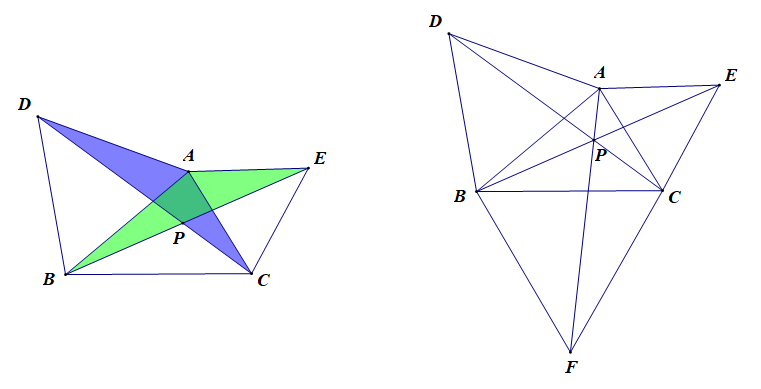
\includegraphics[scale=0.5]{figure/feimadian06}
\end{center}

在上左图中,有$\triangle ADC \cong \triangle ABE$,可得:$CD=BE$.类似的手拉手,在上右图中有3组,可得:$AF=BE=CD$.更巧的是,这三条线段的长度便是我们要求的$PA+PB+PC$的最小值。

我们可以简单的证明如下:

\begin{center}
	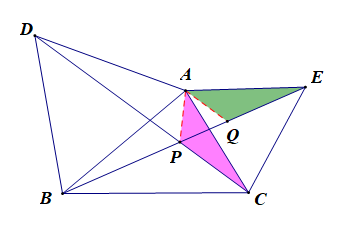
\includegraphics[scale=0.7]{figure/feimadian07}
\end{center}

{\kaishu\color{blue}考虑到$\angle APB=120^\circ$,$\therefore \angle APE=60^\circ$,则可以$AP$为边,在$PE$边取点$Q$使得$PQ=AP$,则$\triangle APQ$是等边三角形.

$\triangle APQ,\triangle ACE$均为等边三角形,且共顶点$A$,故$\triangle APC\cong \triangle AQE$,故有$PC=QE$.

以上两步分别转化$PA=PQ,PC=QE$,故$PA+PB+PC=PB+PQ+QE=BE$}.

总结:从上面的解法可以得出求三角形费马点到三边最小值时({\kaishu 仅仅只求最小值,不要求找到费马点}),\textcolor{red}{只需以三角形某一边向外作等边三角形,然后将等边三角形外面的顶点与原三角形的相对点连接},所得线段的长度即为所求。如下图所示,$BD$即为三角形中任意一点$P$到三个顶点距离之和的最小值。

\begin{center}
	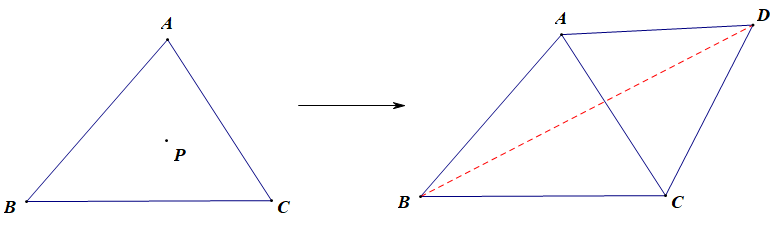
\includegraphics[scale=0.6]{figure/feimadian13}
\end{center}

\section{应用举例}

\begin{shaded}
	\begin{example}
	已知:$\triangle ABC$是等边三角形,$G$为其重心。求证:$GA+GB+GH$最小.
	\end{example}
\end{shaded}

\begin{center}
	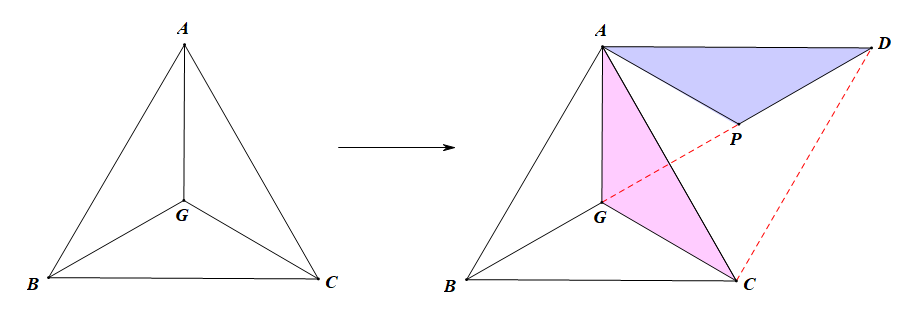
\includegraphics[scale=0.5]{figure/feimadian17}
\end{center}

{\kaishu\color{blue}【证明】将$\triangle AGC$绕点$A$逆时针旋转$60^\circ$,连$GP,CD$.
	
	则 $\triangle AGC\cong \triangle APD$;   
	
	$\therefore \angle APD=\angle AGC=120^\circ,CG=DP,AG=AP, AC=AD,\angle GAC=\angle PAD$.
	
	$\because \angle GAP=60^\circ$,$\therefore  \angle CAD=60^\circ$,
	
	$\therefore  \triangle GAP$和$\triangle CAD$都是等边三角形。
	
	$\because \angle AGB=120^\circ, \angle AGP=60^\circ$.
	
	$\therefore  B,G,P$三点一线。
	
	$\because  \angle APD=120^\circ, \angle APG=60^\circ$.
	
	$\therefore   G,P,D$三点一线。
	
	$\therefore  BG,GP,PD$三条线段同在一条直线上。
	
	$\because GA+GC+GB=GP+PD+GB=BD$.
	
	$\therefore G$点是等腰三角形内到三个顶点的距离之和最小的那一点,即费马点。
}

\begin{shaded}
	\begin{example}
	已知$\triangle ABC$是等腰三角形,$G$是三角形内一点,$\angle AGC=\angle AGB=\angle BGC=120^\circ$。 求证:$GA+GB+GC$最小.	
	\end{example}
\end{shaded}

\begin{center}
	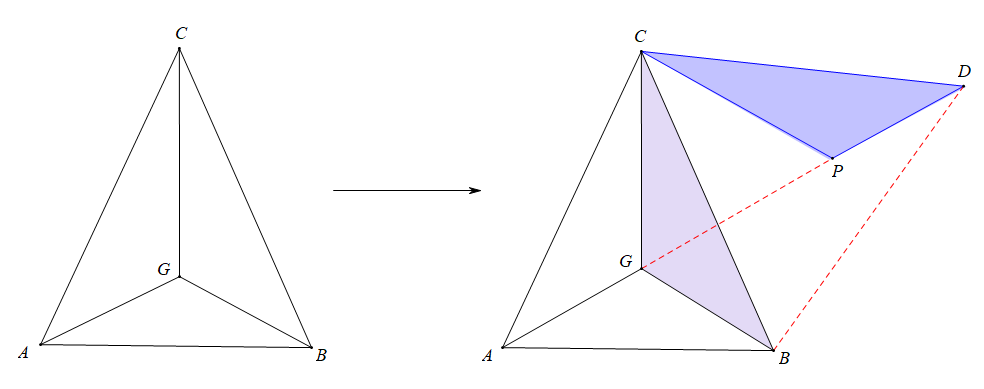
\includegraphics[scale=0.5]{figure/feimadian18}
\end{center}

{\kaishu\color{blue}【证明】将$\triangle BGC$绕点$C$逆时针旋转$60^\circ$,连$GP,DB$.

则 $\triangle CGB\cong \triangle CPD$;   

$\therefore \angle CPD=\angle CGB=120^\circ,CG=CP,GB=PD, BC=DC,\angle GCB=\angle PCD$.

$\because \angle GCP=60^\circ$,$\therefore  \angle BCD=60^\circ$,

$\therefore  \triangle GCP$和$\triangle BCD$都是等边三角形。

$\because \angle AGC=120^\circ, \angle CGP=60^\circ$.

$\therefore  A,G,P$三点一线。

$\because  \angle CPD=120^\circ, \angle CPG=60^\circ$.

$\therefore   G,P,D$三点一线。

$\therefore  AG,GP,PD$三条线段同在一条直线上。

$\because GA+GC+GB=GA+GP+PD=AD$.

$\therefore G$点是等腰三角形内到三个顶点的距离之和最小的那一点,即费马点。
}

\begin{shaded}
	\begin{example}( 广州育才中学2019.5模试题)
	在$\triangle ABC$中,$\angle BAC=90^\circ$,$AB=AC$.
	
	(1)如图1,若$AB=1,BD: CD=1:2$,求$\triangle ABD$的面积;
	
	(2)如图2,若$D$为线段$BC$上任意一点,探究$BD,CD,AD$三者之间的关系,并证明;
	
	(3)如图3,若$AB=1$,$D$为$\triangle ABC$内一点,求$DA+DB+DC$的最小值。
	\end{example}
\end{shaded}

\begin{center}
	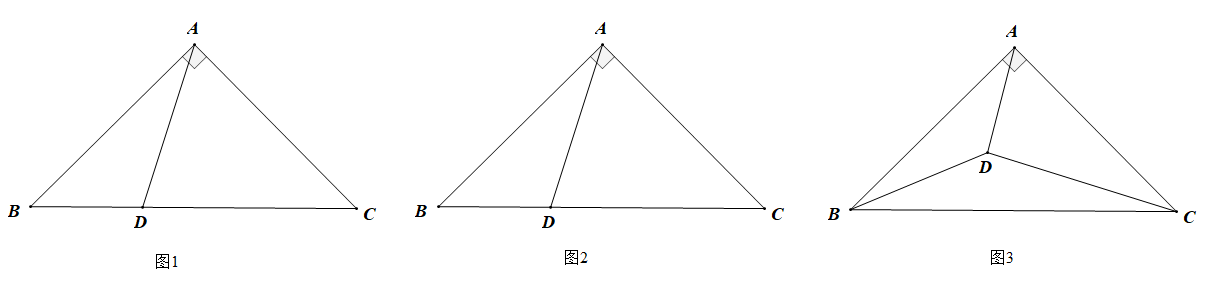
\includegraphics[scale=0.5]{figure/feimadian16}
\end{center}

{\kaishu\color{blue}【 解法一】 如下图,将$\triangle ACD$绕点$A$逆时针旋转$60^\circ$,连接$DP$,则$AD=AP,AC=AE$,又$\angle DAP=60^\circ$,则$DP=AD=AP$,故$DA+DB+DC=DP+BD+PE\geqslant BE$,当$B,D,P,E$四点共线时有最小值,此时$\angle ADB=\angle BDC=\angle ADC=120^\circ$.
过$E$作$EH$垂直$BA$,交$BA$的延长线于$H$.可知$AC=AE=1$,$\angle HAE=30^\circ$,$\therefore EH=\dfrac{1}{2},AH=\dfrac{\sqrt{3}}{2}$.在$Rt\triangle BHE$中,$BE=\sqrt{BH^2+EH^2}=\sqrt{\left(\dfrac{1}{2}\right)^2+\left(1+\dfrac{\sqrt{3}}{2}\right)^2}=\dfrac{\sqrt{6}+\sqrt{2}}{2}$}.

\begin{center}
	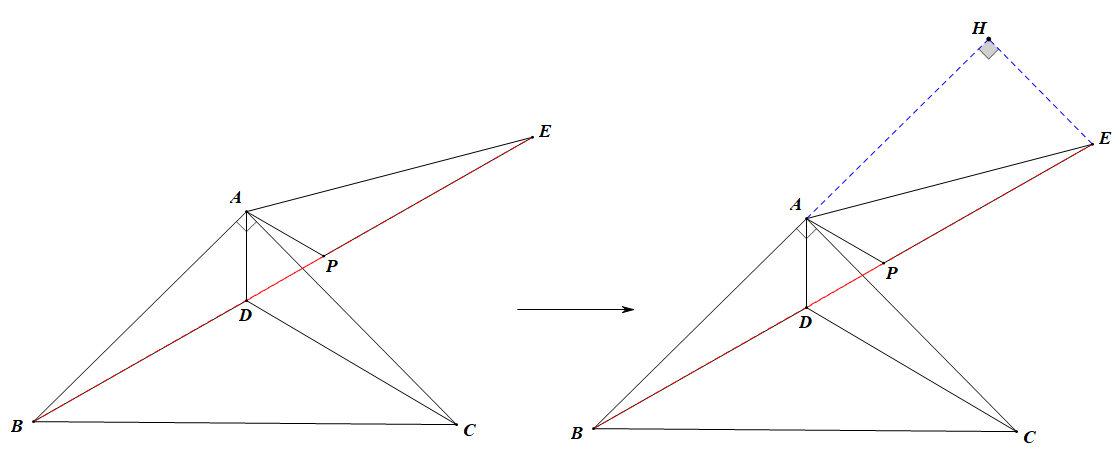
\includegraphics[scale=0.5]{figure/feimadian21}
\end{center}

{\kaishu\color{blue}【 解法二】 如下图,以$AC$为边向外作等边$\triangle ACE$,连接$BE$,则$BE$即为所求.过$E$作$EH$垂直$BA$,交$BA$的延长线于$H$.可知$AC=AE=1$,$\angle HAE=30^\circ$,$\therefore EH=\dfrac{1}{2},AH=\dfrac{\sqrt{3}}{2}$.在$Rt\triangle BHE$中,$BE=\sqrt{BH^2+EH^2}=\sqrt{\left(\dfrac{1}{2}\right)^2+\left(1+\dfrac{\sqrt{3}}{2}\right)^2}=\dfrac{\sqrt{6}+\sqrt{2}}{2}$}.

\begin{center}
	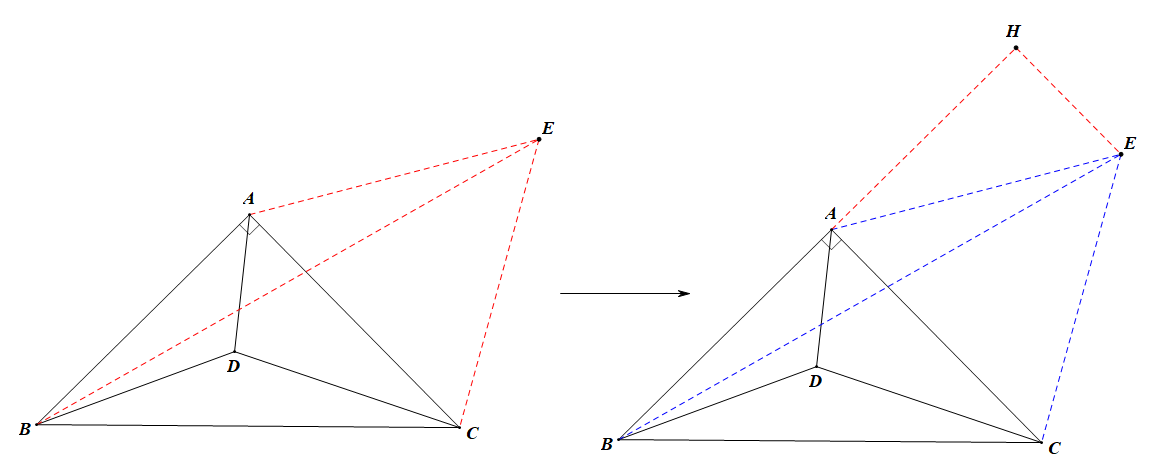
\includegraphics[scale=0.5]{figure/feimadian20}
\end{center}


\section{习题演练}
\begin{shaded}
1.如图,在$\triangle ABC$中,$\angle ACB=90^\circ$,$BC=AC=\sqrt{2}$,$P$是$\triangle ABC$内一点,求$PA+PB+PC$的最小值.
\end{shaded}

\begin{center}
	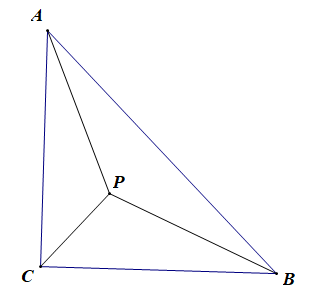
\includegraphics[scale=0.5]{figure/feimadian14}
\end{center}

\begin{shaded}
2.如图,已知矩形$ABCD$,$AB=4$,$BC=6$,点$M$为矩形内一点,点$E$为$BC$边上任意一点,则$MA+MD+ME$的最小值为$\underline{\hspace{1.5cm}}$.
\end{shaded}

\begin{center}
	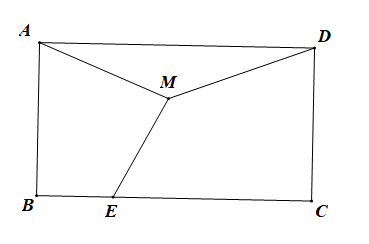
\includegraphics[scale=0.5]{figure/feimadian15}
\end{center}

\begin{shaded}
3.$\triangle ABC$中,点$D$是费马点,$\angle ABC=60^\circ$,$AD=3,CD=4$,求$BD$的长.
\end{shaded}

\begin{center}
	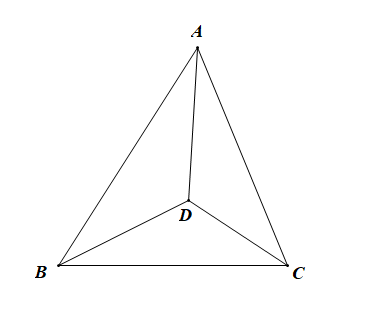
\includegraphics[scale=0.5]{figure/feimadian25}
\end{center}

\begin{shaded}
4.如图,在$\triangle ABC$中,$\angle ABC=60^\circ$,$AB=5$,$BC=3$,$P$是$\triangle ABC$内一点,求$PA+PB+PC$的最小值,并确定当$PA+PB+PC$取得最小值时,$\angle APC$的度数.
\end{shaded}

\begin{center}
	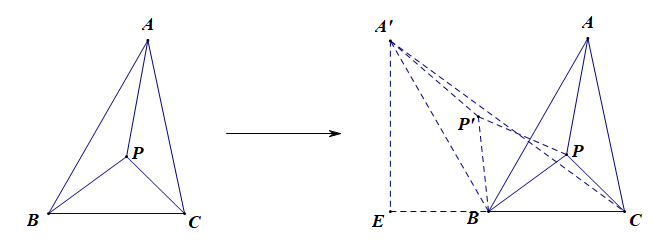
\includegraphics[scale=0.6]{figure/feimadian10}
\end{center}

\begin{shaded}
5.(2010福建宁德中考)如图,四边形$ABCD$是正方形,$\triangle ABE$是等边三角形,$M$为对角线$BD$上任意一点,将$BM$绕点$B$逆时针旋转$60^\circ$得到$BN$,连结$AM,CM,EN$.

(1)当$M$在何处时,$AM+CM$的值最小?

(2)当$M$在何处时,$AM+BM+CM$的值最小?请说明理由;

(3)当$AM+BM+CM$的最小值为$\sqrt{3}+1$时,求正方形的边长.
\end{shaded}

\begin{center}
	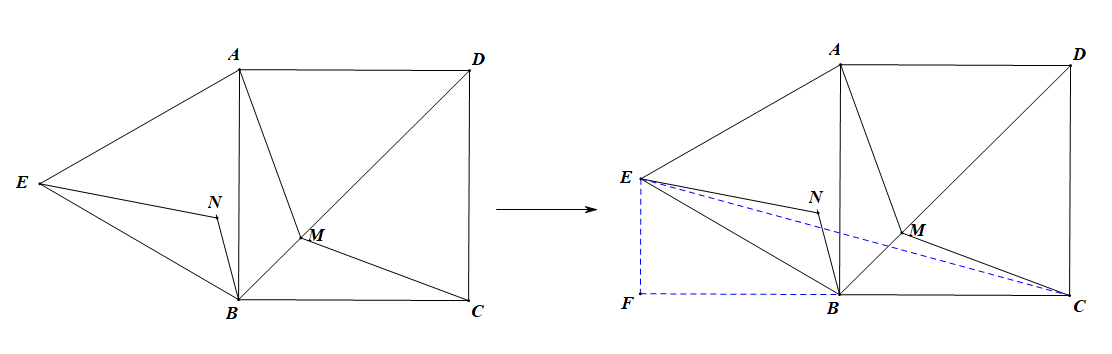
\includegraphics[scale=0.5]{figure/feimadian09}
\end{center}

\begin{shaded}
6.(2008年广东中考题)已知正方形$ABCD$内一动点$E$到$A$、$B$、$C$三点的距离之和的最小值为$\sqrt{2}+\sqrt{6}$,求此正方形的边长.
\end{shaded}

\begin{center}
	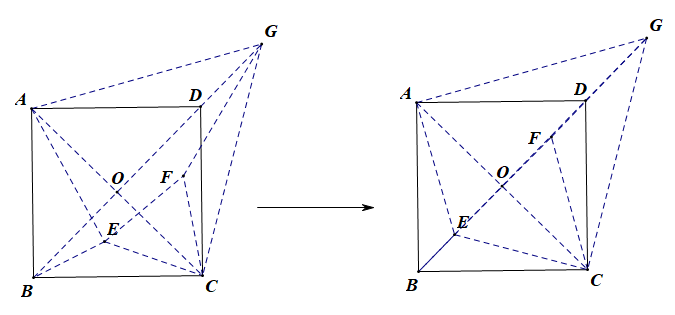
\includegraphics[scale=0.6]{figure/feimadian11}
\end{center}

分析:连接$AC$,发现点$E$到$A$、$B$、$C$三点的距离之和就是到$\triangle ABC$三个顶点的距离之和,这实际是费尔马问题的变形,只是背景不同.
解   如图2,连接$AC$,把$\triangle AEC$绕点$C$顺时针旋转$60^\circ$,得到$\triangle GFC$,连接$EF$、$BG$、$AG$,可知$\triangle EFC,\triangle AGC$都是等边三角形,则$EF=CE$.
又$FG=AE$,
$\therefore AE+BE+CE = BE+EF+FG($
$\because$点$B$、点$G$为定点( $G$为点$A$绕$C$点顺时针旋转$60^\circ$所得). 
$\therefore$线段$BG$即为点$E$到$A,B,C$三点的距离之和的最小值,此时$E,F$两点都在$BG$上(图3).
设正方形的边长为$a$,那么
$BO=CO=\dfrac{\sqrt{2}}{2}a,GC=\sqrt{2}a, GO=\dfrac{\sqrt{6}}{2}a$.
$\therefore BG=BO+GO =\dfrac{\sqrt{2}}{2}a+\dfrac{\sqrt{6}}{2}a$.
$\because$点$E$到$A,B,C$三点的距离之和的最小值为$\sqrt{2}+\sqrt{6}$.
$\therefore \dfrac{\sqrt{2}}{2}a+\dfrac{\sqrt{6}}{2}a=\sqrt{2}+\sqrt{6}$,解得$a=2$.

\vspace{1cm}

\begin{shaded}
7.(2009年北京中考题) 如图 ,在平面直角坐标系$xOy$中,$\triangle ABC$三个顶点的坐标分别为$A(-6,0),B(6,0),\\
C(0,4\sqrt{3})$,延长$AC$到点$D$, 使$CD=\dfrac{1}{2}AC$,过点$D$作$DE//AB$交$BC$的延长线于点$E$.

(1)求$D$点的坐标;     
                         
(2)作$C$点关于直线$DE$的对称点$F$,分别连结$DF,EF$,若过$B$点的直线$y=kx+b$将四边形$CDFE$分成周长相等的两个四边形,确定此直线的解析式;

                         
(3)设$G$为$y$轴上一点,点$P$从直线$y=kx+b$与$y$轴的交点出发,先沿$y$轴到达$G$点,再沿$GA$到达$A$点,若$P$点在$y$轴上运动的速度是它在直线$GA$上运动速度的2倍,试确定$G$点的位置,使$P$点按照上述要求到达$A$点所用的时间最短(要求:简述确定$G$点的方法,但不要求证明).
\end{shaded}

\begin{center}
	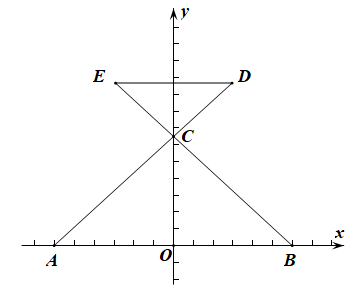
\includegraphics[scale=0.6]{figure/feimadian27}
\end{center}

\vspace{1cm}

\begin{shaded}
8.(2009年湖州中考题)若点$P$ 为$\triangle ABC$所在平面上一点,且$\angle APB=\angle BPC=\angle CPA=120^\circ$, 则点$P$叫做$\triangle ABC$的费马点.

(1)若$P$为锐角$\triangle ABC$的费马点,且$\angle ABC=60^\circ$,$PA=3,PC=4$, 则$PB$的值为$\underline{\hspace{1.5cm}}$;

(2)如图,在锐角$\triangle ABC$的外侧作等边$\triangle ACB′$,连结$BB′$.求证:$BB′$ 过$\triangle ABC$的费马点$P$,且$BB′=PA+PB+PC$.
\end{shaded}

\begin{center}
	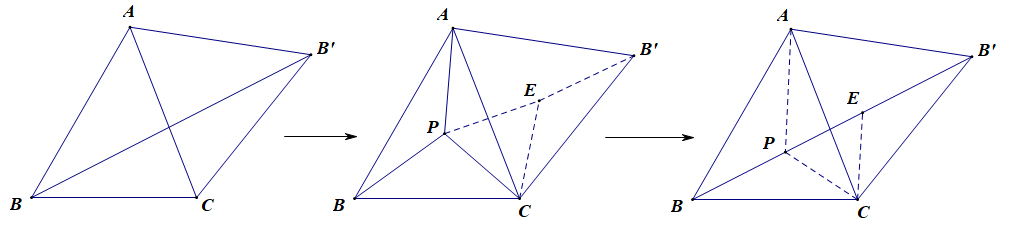
\includegraphics[scale=0.5]{figure/feimadian12}
\end{center}

\begin{shaded}
9.(2019武汉中考题)问题背景:如图1,将$\triangle ABC$绕点$A$逆时针旋转$60^\circ$得到$\triangle ADE$,$DE$与$BC$交于点$P$,可推出结论:$PA+PC=PE$.

问题解决:如图2,在$\triangle MNG$中,$MN=6$,$\angle M=75^\circ$,$MG=4\sqrt{2}$,点$O$是$\triangle MNG$内一点,则点$O$到$\triangle MNG$三个顶点的距离和的最小值是$\underline{\hspace{1.5cm}}$.
\end{shaded}

\begin{center}
	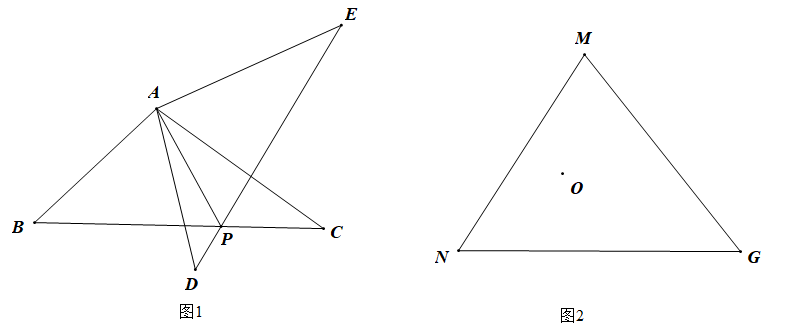
\includegraphics[scale=0.5]{figure/feimadian26}
\end{center}

\begin{shaded}
10.(广州市第五中学2019.11期中)已知,如图,$\triangle ABC$的三条边$BC=a$,$CA=b$,$AB=c$,$D$为内一点,且$\angle ADB=\angle BDC=\angle CDA=120^\circ$,$DA=u$,$DB=v$,$DC=w$.

(1)若$\angle CBD=18^\circ$,则$\angle BCD=$$\underline{\hspace{1.5cm}}$;

(2)将$\triangle ACD$绕点$A$顺时针旋$90^\circ$转到$\triangle AC'D'$,画出$\triangle AC'D'$,若$\angle CAD=20^\circ$,求$\angle CAD'$度数;

(3)试画出符合下列条件的正三角形:$M$为正三角形内的一点,$M$到正三角形三个顶点的距离分别为$a,b,c$,且正三角形的边长为$u+v+w$,并给予证明。
\end{shaded}

\begin{center}
	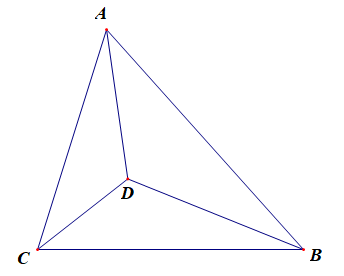
\includegraphics[scale=0.5]{figure/feimadian28}
\end{center}

\vspace{1cm}

\begin{shaded}
11.(2016 朝阳中考)小颖在学习“两点之间线段最短”查阅资料时发现:$\triangle ABC$内总存在一点$P$与三个顶点的连线的夹角相等,此时该点到三个顶点的距离之和最小.
\end{shaded}

\begin{center}
	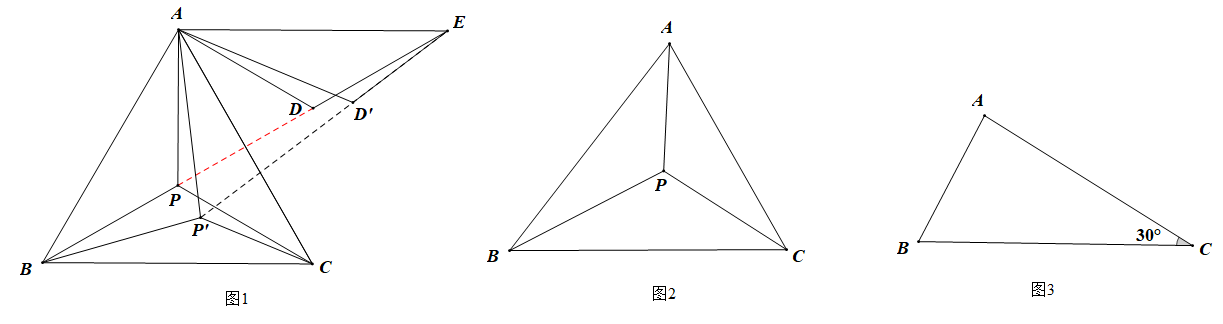
\includegraphics[scale=0.5]{figure/feimadian22}
\end{center}

\begin{shaded}
【特例】如图1,点$P$为等边$\triangle ABC$的中心,将$\triangle ACP$绕点$A$逆时针旋转$60^\circ$得到$\triangle ADE$,从而有$DE=PC$.连接$PD$得到$PD=PA$,同时$\angle APB+\angle APD=120^\circ+60^\circ=180^\circ$,$\angle ADP+\angle ADE=120^\circ+60^\circ=180^\circ$,即$B,P,D,E$四点共线,故$PA+PB+PC=PD+PB+DE=BE$.

在$\triangle ABC$中,另取一点$P'$,易知点$P'$与三个顶点连线的夹角不相等,可证明$B,P',D',E$四点不共线,所以$P'A+P'B+P'C>PA+PB+PC$,即点$P$到三个顶点距离之和最小.

【探究】(1)如图2,$P$为$\triangle ABC$内一点,$\angle APB=\angle BPC=120^\circ$,证明:$PA+PB+PC$的值最小.

【拓展】(2)如图3,$\triangle ABC$中,$AC=6,BC=8,\angle ACB=30^\circ$,且点$P$为$\triangle ABC$内一点,求$P$到三个顶点的距离之和的最小值.
\end{shaded}

\vspace{1cm}

\begin{shaded}
12.( 朝阳二模)小华遇到这样一个问题,如图1,$\triangle ABC$中,$\angle ACB=30^\circ,BC=6,AC=5$,在$\triangle ABC$内部有一个点$P$,连接$PA,PB,PC$,求$PA+PB+PC$的最小值.
\end{shaded}

\begin{center}
	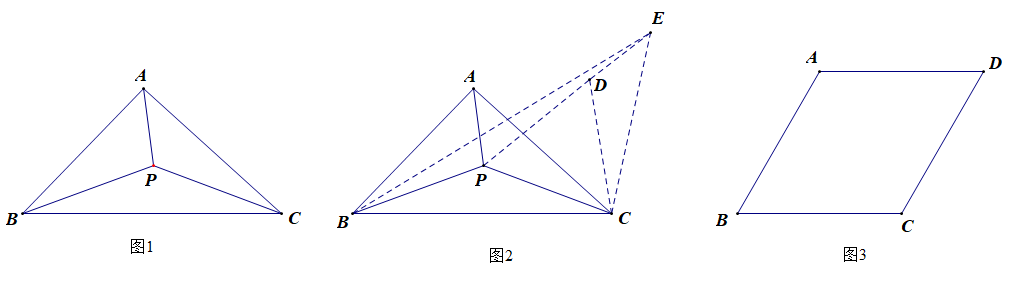
\includegraphics[scale=0.5]{figure/feimadian23}
\end{center}

\begin{shaded}
小华是这样思考的:要解决这个问题,首先应想办法将这三条端点重合于一点的线段分离,然后再将它们连接一条折线,并让折线的两个端点为定点,这样依据“两点之间线段最短”,就可以求出这三条线段和的最小值了.他先后尝试了翻折、旋转、平移的方法,发现通过旋转可以解决这个问题.他的做法是,如图2,将$\triangle APC$绕点$C$顺时针$60^\circ$,得到$\triangle EDC$,连接$PD,BE$,则$BE$的长即为所求.

(1)请你写出图2中,$PA+PB+PC$的最小值为$\underline{\hspace{1.5cm}}$.

(2)参考小华的思考问题的方法,解决下列问题:

\ding{192}如图3,菱形$ABCD$中,$\angle ABC=60^\circ$,在菱形$ABCD$内部有一点$P$,请在图3中画出并指明长度等于$PA+PB+PC$最小值的线段(保留画出痕迹,画出一条即可);

\ding{193}若\ding{192}中菱形$ABCD$的边长为4,请直接写出当$PA+PB+PC$值最小时$PB$的长.
\end{shaded}

\vspace{1cm}

\begin{shaded}
13.( 延庆中考题)阅读下面材料:
小伟遇到这样一个问题:如图1,在$\triangle ABC$(其中$\angle BAC$是一个可以变化的角)中,$AB=2$,$AC=4$,以$BC$为边在$BC$的下方作等边$\triangle PBC$,求$AP$的最大值;
\end{shaded}

\begin{center}
	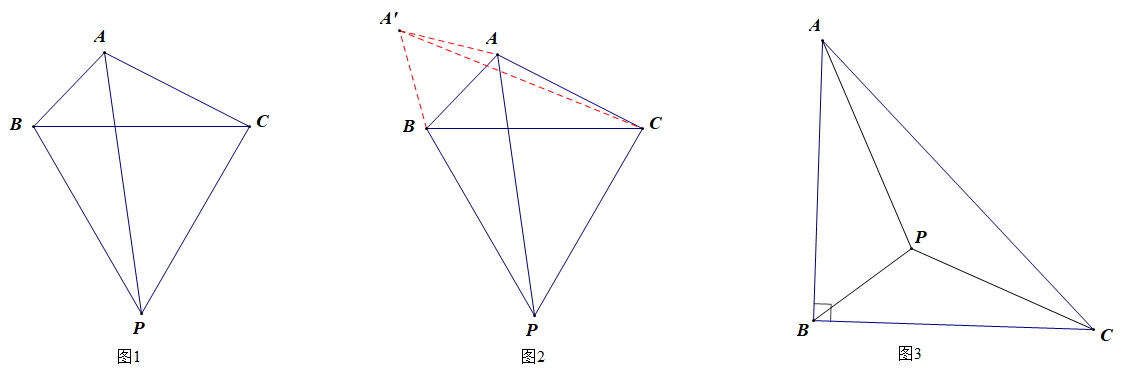
\includegraphics[scale=0.5]{figure/feimadian24}
\end{center}

\begin{shaded}
小伟是这样思考的:利用变换和等边三角形将边的位置重新组合,他的方法是以点$B$为旋转中心将$\triangle ABP$逆时针旋转$60^\circ$得到$\triangle A'BC$,连接$AA'$,当点$A$落在$A'C$上时,此题可解(如图2).

请你回答:$AP$的最大值是$\underline{\hspace{1.5cm}}$.

参考小伟同学思考问题的方法,解决下列问题:
如图3,等腰$Rt\triangle ABC$,边$AB=4$,$P$为$\triangle ABC$内部一点,则$AP+BP+CP$的最小值是$\underline{\hspace{1.5cm}}$(结果可以不化简).
\end{shaded}

\vspace{1cm}

\begin{shaded}
14.如图,在平面直角坐标系$xOy$中,点$B$的坐标为$(0,2)$,点$D$在$x$轴的正半轴上,$\angle ODB=30^\circ,OE$为$\triangle BOD$的中线.过$B,E$两点的抛物线$y=ax^2+\dfrac{\sqrt{3}}{6}x+c$与$x$轴相交于$A,F$两点($A$在$F$的左侧)。

(1)求抛物线的解析式;

(2)等边$\triangle OMN$的顶点$M,N$在线段$AE$上,求$AE$及$AM$的长;

(3)点$P$为$\triangle ABO$内的一个动点,设$m=PA+PB+PO$,请直接写出$m$的最小值,以及$m$取得最小值时,线段$AP$的长。
\end{shaded}

\begin{center}
	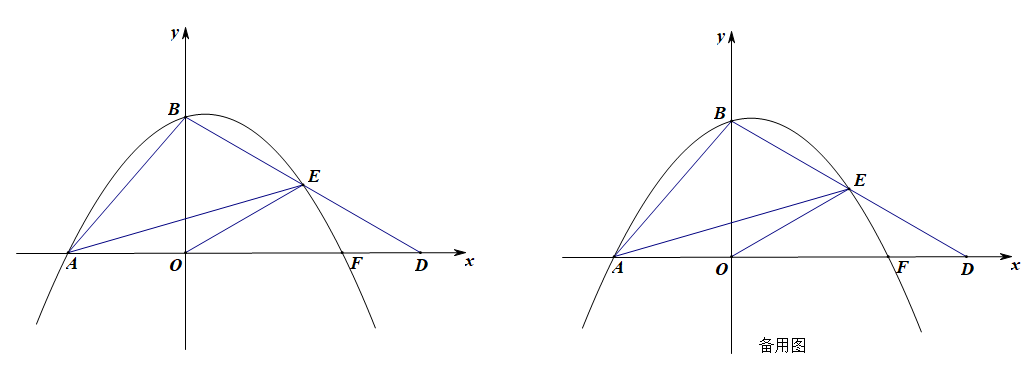
\includegraphics[scale=0.6]{figure/feimadian08}
\end{center}

















\end{document}